

En este capítulo, vamos a utilizar el Horiba PTI QM 400 renovado y con su ampliación de capacidades para realizar mediciones de espectros estáticos de excitación y emisión, así como mediciones de tiempo de vida.
En la primera sección vamos a medir y comparar los espectros estacionarios de la rodamina B usando el instrumento renovado y el original.
En la segunda sección vamos a caracterizar ópticamente un lote de UCNPs.
Todas las partículas usadas en este trabajo fueron sintetizadas por el equipo colaborador del INQUIMAE, liderado por Beatriz Barja y María Claudia Marchi. 
Las nanopartículas utilizadas consisten en una red cristalina de fluoruro de ítrio NaYF$_4$ dopadas con los lantánidos iterbio (Yb) y erbio (Er), que en conjunto conforman una de las UCNPs más eficientes descriptas hasta el momento NaYF$_4$:Yb$^{+3}$,Er$^{+3}$ \cite{caracterizacion_ucnps_unicas}.
El método de síntensis empleado escapa el alcance de esta tésis, pero está detalladamente documentado en la literatura \cite{Zhang2012}.

\section{Espectros estacionarios de la rodamina B}

La rodamina es un fluoróforo extensamente usado en microscopía de fluorescencia debido a su fotoestabilidad y sus propiedades fotofísicas \cite{beija_synthesis_2009,rodamina_caracterizacion}.
Debido a su popularidad, sus espectros de excitación y emisión así como sus métodos de síntesis son ampliamente conocidos y reproducibles.
En particular, se caracteriza por tener un pico en 551 nm para la absorción y uno en 576 nm para la emisión.
A modo de verificación de que la medición de un espectro estático, tanto de excitación como de emisión, es el mismo utilizando el \textit{software} y el \textit{hardware} renovado y el original, medimos el espectro de la rodamina B.
Para eso Marcos Illescas, integrante del grupo de fotofísica del INQUIMAE, preparó una muestra de rodamina B disuelta en etanol.
Dado que el objetivo es comparar el espectro medido con el instrumento original y el renovado no se registraron las concentraciones ni la pureza de la solución.
La muestra se colocó en una cubeta y luego en el portacubetas de la cámara de muestras del fluorímetro.
Para el espectro de emisión se realizó la excitación con la lámpara de xenón original del instrumento a una longitud de onda fija de 520 nm y un barrido de emisión entre 530 y 700 nm.
Para el espectro de excitación se realizó un barrido de 420 a 590 nm, observando la intensidad de luz emitida a 600 nm.


En la figura (\textbf{\ref{fig:rodamina}}) se ven los cuatro espectros normalizados por su máximo de intensidad.
Se puede ver que los espectros medidos con el instrumento original (azul) se solapan completamente con los medidos con nuestra renovación (naranja).
Dado que las transiciones electrónicas presentes en la rodamina son dipolares sus tiempos de vida medios son del orden de los nanosegundos, por lo que son imposibles de medir con nuestro instrumento con resolución mínima de $\sim 100$ ns.
En la siguiente sección utilizamos el espectrofluorímetro renovado para su propósito inicial: la caracterización óptica de UCNPs.

\begin{SCfigure}
    \centering
    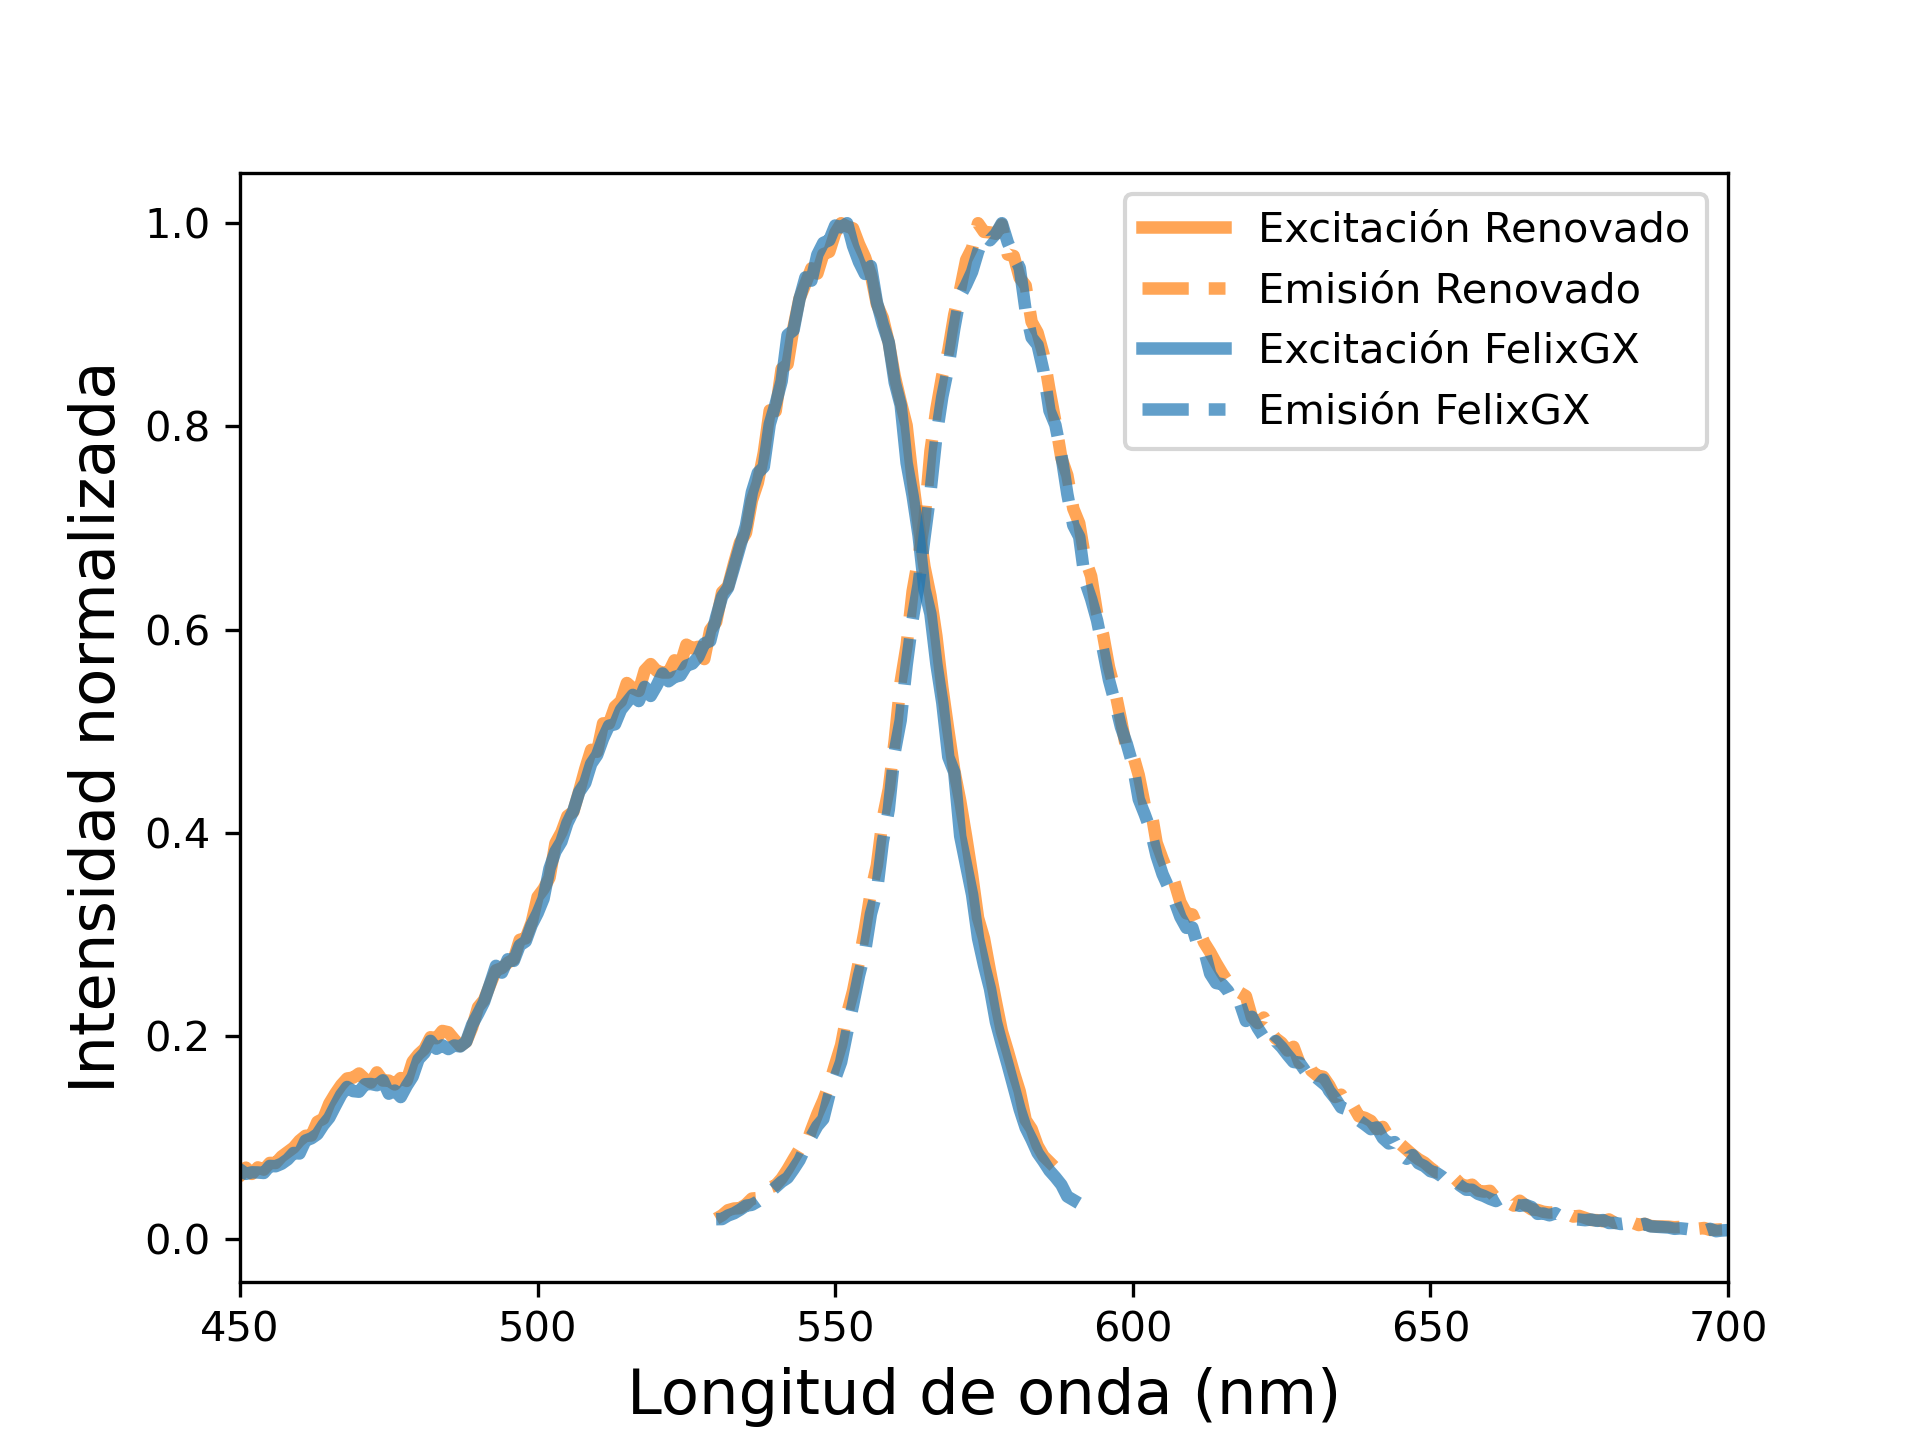
\includegraphics[width=0.7\textwidth]{rho6b_validacion.png}
    \caption{\textbf{Espectros de la rodamina B}, tanto de excitación (punteado) como de emisión (sólido). Ambos fueron medidos con el \textit{software} y \textit{hardware} original (azul) como con el renovado (naranja).}
    \label{fig:rodamina}
\end{SCfigure}

\section{Caracterización óptica de UCNPs}

\begin{figure}
    \centering
    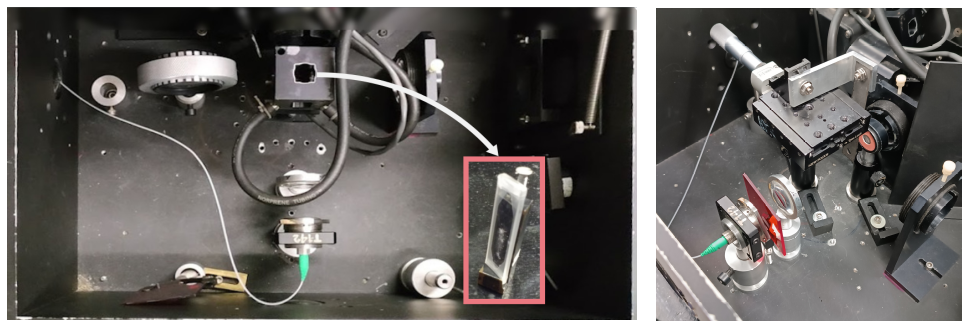
\includegraphics[width=\textwidth]{camara_muestra.png}
    \caption{\textbf{Imagen de la cámara de la muestra}. (izquierda) Se ve la cámara del fluorímetro sin filtro. Recuadrado en rosa hay una foto de la muestra sobre el sujetador. (derecha) Se ve el arreglo para medir el perfil del haz. En esta foto se ve el filtro utilizado en las mediciones.}
    \label{fig:camara_muestra}
\end{figure}

\begin{figure}
    \centering
    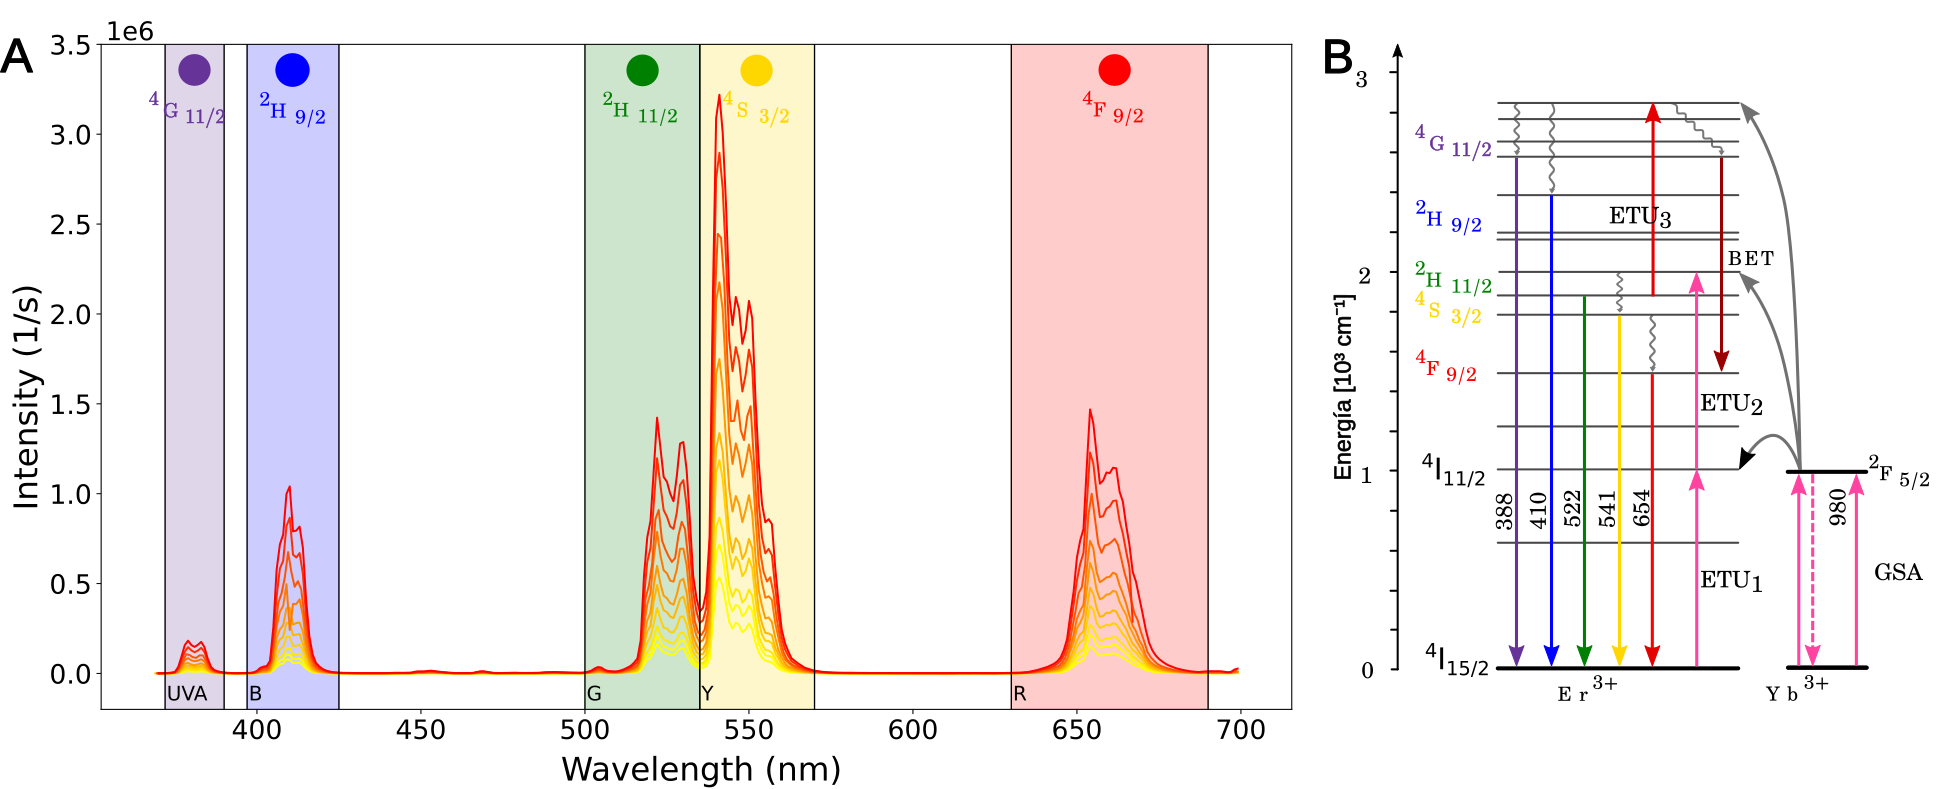
\includegraphics[width=\textwidth]{spectrum_powerdens.png}
    \caption{\textbf{Espectro de las UCNPs dependiente de la potencia.} (A) Espectro de emisión bajo excitación CW por un diodo láser de 976 nm para distintas densidades de potencia de excitación entre 16 mW cm$^{-2}$ y 80 mW cm$^{-2}$.
    (B) Esquema de niveles de Yb$^{+3}$ y Er$^{+3}$, marcados con colores los niveles excitados del Er$^{+3}$ cuya emisión corresponde a las regiones del espectro.}
    \label{fig:power_dep_spectrum}
\end{figure}

Nuestra plataforma adaptada nos permitió medir el espectro dinámico dependiente de la potencia de las UCNPs sintetizadas (\textbf{Fig. \ref{fig:power_dep_spectrum}}), y sus tiempos de vida (\textbf{Fig. \ref{fig:lifetimes}}) al ser excitadas con un láser de diodo IR de 976 nm.  
La muestra utilizada consta de un polvo de UCNP depositado sobre un portamuestras.
Sostuvimos al portamuestras con un sujetador que luego se coloca en el portacubetas de la cámara (\textbf{Fig. \ref{fig:camara_muestra}}).
El láser externo se acopla a fibra y luego se enfoca con una lente sobre la muestra.
Para poder medir en un rango amplio de densidades de potencia con la misma configuración se colocó un filtro atenuador entre la salida de la fibra y la lente.
Esto nos permitió configurar altas potencias de excitación sin que sature la detección de fotones.
Dado que la adquisición de los datos tomó muchos días, se aseguró el sujetador al portacubetas con cinta adhesiva para poder reproducir las mediciones y no se movió hasta tomar todos los espectros.
Por último, se midió el perfil de intensidad del haz en el foco de la lente.
Para eso se utilizó una cuchilla montada a un micrómetro que tapaba el haz que incidía sobre un medidor de potencia.
Se graficó la intensidad en función de la posición de la cuhilla.
Asumiendo que el perfil es gaussiano se ajustó por la función error y se obtuvo un área de $(1.5 \pm 0.1)$ cm$^2$ \footnote{Todos los códigos de análisis se encuentran en el archivo \texttt{analysis\_paper.ipynb} de \href{https://github.com/tdinapoli/tesis}{https://github.com/tdinapoli/tesis}}.

\begin{figure}
    \centering
    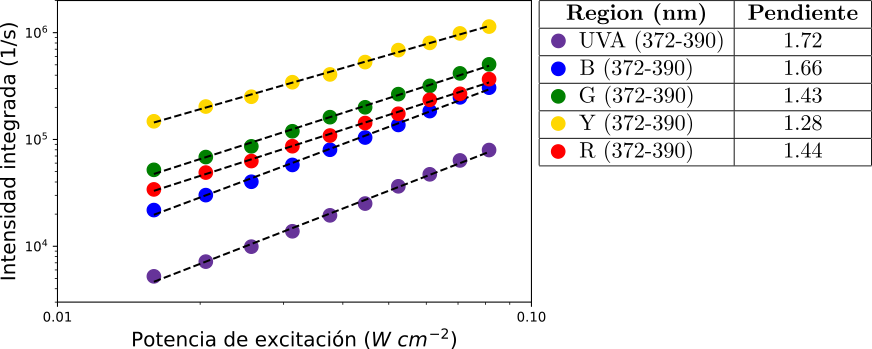
\includegraphics[width=\textwidth]{power_dep_ranges.png}
    \caption{\textbf{Gráfico Log-Log de I vs. P.} Codificado con colores se encuentran las intensidades para cada potencia de excitación para cada uno de las regiones del espectro definidas. La tabla muestra la pendiente de un ajuste lineal para cada rango.}
    \label{fig:power_dep_ranges}
\end{figure}

Como fue detallado en la sección \ref{sec:intro_ucnp}, la conversión ascendente es un proceso óptico no lineal en el que dos o más fotones se absorben secuencialmente entre niveles de energía igualmente espaciados, lo que lleva a la emisión de luz con una longitud de onda más corta que la incidente.  
Debido a las particularmente largas vidas medias (del orden de los cientos de microsegundos) y a los niveles de energía escalonados de los iones de tierras raras, se pueden observar espectros de conversión ascendente de UCNP en el rango visible incluso a bajas potencias de excitación.  
En este caso, medimos los espectros estáticos con densidades de potencia que varían entre 16 mW cm$^{-2}$ y 80 mW cm$^{-2}$ al excitar con el láser de forma continua (CW) (\textbf{Fig. \ref{fig:power_dep_spectrum}A}).  
El espectro estático muestra los picos de emisión conocidos de los iones Er$^{3+}$, que van desde la energía más baja hasta la más alta del espectro visible.  
Comenzando por el lado de menor energía, etiquetamos las regiones de emisión como rojo (R, 630–690 nm), amarillo (Y, 535–570 nm) y verde (G, 500–535 nm), correspondientes a las transiciones $^4$F$_{9/2} \to ^4$I$_{15/2}$, y $^4$S$_{3/2}, ^2$H$_{11/2} \to ^4$I$_{15/2}$, respectivamente.  
El espectro también muestra azul (B, 397–425 nm) y ultravioleta (UVA, 372–390 nm), que provienen de transiciones de niveles excitados más altos, como $^2$H$_{9/2} \to ^4$I$_{15/2}$ (410 nm) o $^4$G$_{11/2} \to ^4$I$_{15/2}$ (383 nm) \cite{haase_upconverting_2011}.  
Como se mencionó en la sección \ref{sec:intro_ucnp}, aunque las UCNPs muestran una relación no lineal entre la intensidad de emisión y la densidad de potencia de excitación, esto solo es apreciable cuando se abarcan varios órdenes de magnitud \cite{pollnau2000}.  
La intensidad de emisión de conversión ascendente ($I_{UC}$) está relacionada de manera no lineal con la densidad de potencia de excitación, $I_{UC} = P^\alpha$, donde $\alpha$ es el número efectivo de fotones involucrados en el proceso de absorción por fotón de mayor energía emitido, y $P$ es la potencia incidente \cite{Auzel2004}.  
El gráfico $\log{(I_{UC})}$ vs. $\log{(P)}$ (\textbf{Fig. \ref{fig:power_dep_ranges}}) muestra que, para este rango de potencias, cada región de emisión está caracterizada por una pendiente relacionada con el número de fotones involucrados en cada proceso (\textbf{Fig. \ref{fig:power_dep_ranges} inset}).  
No se observaron cambios en estas pendientes para cada longitud de onda (UV, B, G, R), lo que indica que los mecanismos fotofísicos que causan la conversión ascendente son los mismos para todas las potencias.  
Esto está en línea con el hecho de que la relajación cruzada y la transferencia de energía hacia atrás (BET) desde Er$^{3+}$ hacia Yb$^{3+}$ son despreciables en estos límites de baja potencia \cite{suyver_anomalous_2005} \cite{berry_disputed_2015}.


\begin{figure}[t]
    \centering
    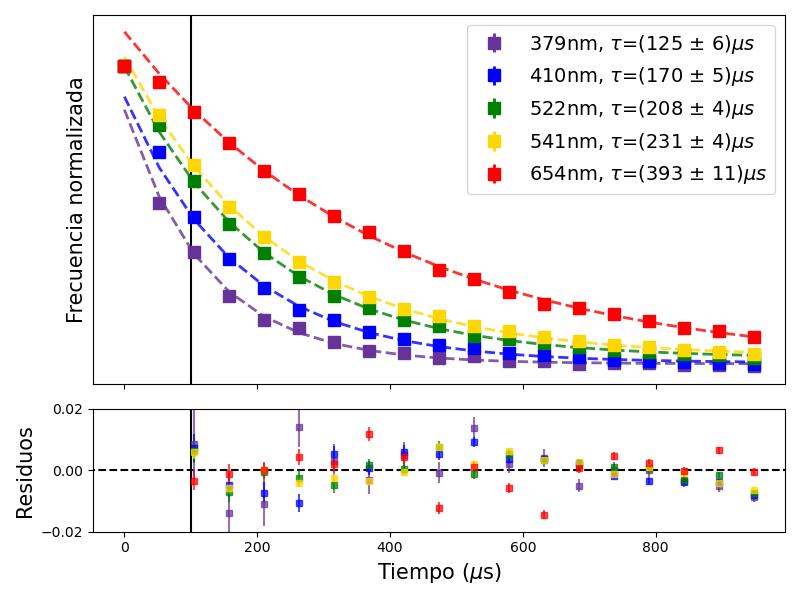
\includegraphics[width=\textwidth]{lifetimes_residuos.png}
    \caption{\textbf{Histogramas de tiempos de vida.} Tiempo de arribo de los fotones (cuadrados) y ajuste de decaimiento exponencial (líneas sólidas) para cada región del espectro. Los tiempos de vida se midieron a 976 nm, 0.087 mW cm$^{-2}$.}
    \label{fig:lifetimes}
\end{figure}

Además de obtener los espectros estacionarios de las UCNPs, medimos el tiempo de vida medio en los picos de emisión de cada una de las regiones espectrales (\textbf{Fig. \ref{fig:lifetimes}}), esto es para las longitudes de onda 379, 410, 522, 541 y 654 nm.
Ajustamos los histogramas de tiempo de arribo de los fotones con una curva de decaimiento monoexponencial, comenzando a los 100 $\mu$s después de que se detuvo la excitación para medir solo la desocupación de los estados excitados.  
El resultado son vidas medias que varían entre $\sim125$ y $\sim400$ $\mu$s.  
Se observa una disminución en la vida media para los fotones de longitud de onda más corta, correspondientes a estados excitados de mayor energía, lo que es consistente con un mayor número de vías de relajación. 
Por otro lado, se puede ver que los residuos no están uniformemente distribuidos.
Esto es esperable, ya que el modelo de decaimiento monoexponencial es un modelo efectivo para el comportamiento.
Como comentamos en la sección \ref{sec:intro_ucnp}, el modelo más completo para la dinámica de las UCNP consiste en 12 ecuaciones diferenciales ordinarias no lineales, con $\sim 50$ parámetros libres, en cambio nuestro modelo efectivo tiene un solo parámetro.
Adicionalmente, medimos el tiempo de vida para el pico de emisión de 541 nm a dos potencias distintas de excitación, 3 y 87 mW \textbf{\ref{fig:lifetimes_power}}.
Al igual que con la relación entre potencia e intensidad, el cambio en tiempo de vida no presenta diferencias significativas para el rango de potencias en el que medimos.

Para este rango de potencias de excitación, no se llegan a medir diferencias significativas ni en la relación funcinoal entre potencia e intensidad, ni en el tiempo de vida para el pico más intenso de emisión.
En el futuro, se podrían repetir las mediciones excitando a densidades de potencia en el rango de 10$^0$ mW cm$^{-2}$ y 10$^2$ mW cm$^{-2}$, en el que se observan cambios en la pendiente de los gráficos $\log(I)$ vs. $\log(P)$ \cite{bujjamer_luminescent_2020}.
Sin embargo, estas mediciones demuestran la posibilidad de realizar una caracterización óptica completa de las nanopartículas de \textit{upconversion} con las modificaciones que realizamos en el espectrofluorímetro QM 400.
Tanto las mediciones de espectro en función de la potencia como las de tiempo de vida fueron realizadas automáticamente con secuencias de comandos programadas en Python.
La plataforma permite desarrollar una secuencia de comandos más compleja que mida un espectro completo, detecte los picos de emisión y mida los tiempos de vida en esos picos, de forma que el usuario sólo tendría que colocar la muestra en la cámara y ejecutar el programa para realizar una caracterización óptica completa.




\begin{SCfigure}
    \centering
    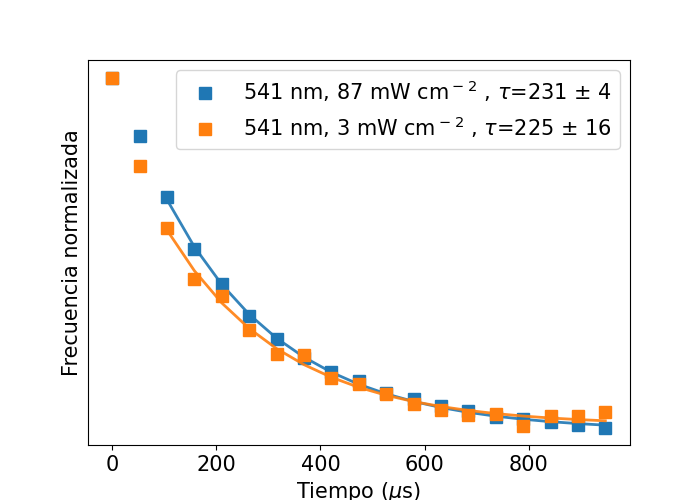
\includegraphics[width=0.7\textwidth]{lifetimes_power.png}
    \caption{\textbf{Tiempo de vida a distintas potencias.} Tiempo de arribo de los fotones (cuadrados) para el pico de emisión de 541 nm y dos potencias de excitación distintas, 3 mW cm$^{-2}$ y 87 mW cm$^{-2}$.}
    \label{fig:lifetimes_power}
\end{SCfigure}
